
%(BEGIN_QUESTION)
% Copyright 2012, Tony R. Kuphaldt, released under the Creative Commons Attribution License (v 1.0)
% This means you may do almost anything with this work of mine, so long as you give me proper credit

Protective relays are typically found only in electric power grid applications, or at industrial facilities where exceptionally large loads are operated (e.g. huge motors for ball mills, compressors, pumps, etc.).  However, there is a type of circuit protective device that is so common, it exists within almost every home in the United States: a {\it Ground Fault Current Interruptor}, or {\it GFCI}.

The basic idea behind a GFCI is represented in this simplified schematic diagram:

$$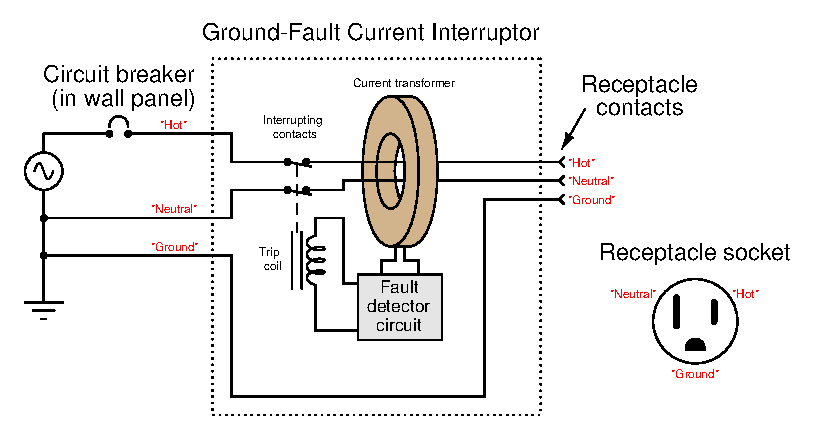
\includegraphics[width=15.5cm]{i01201x01.eps}$$

A GFCI receptacle uses a single current transformer (CT) to measure the {\it difference} in electric current through the ``hot'' and ``neutral'' conductors of any electrical appliance plugged into the receptacle.  If even a slight difference is detected, the interruptor contacts open, stopping power to the appliance.

\vskip 10pt

Explain how a single CT is able to detect a difference in current between two conductors.  Also, explain how a difference in current would ever arise between the ``hot'' and ``neutral'' conductors of an appliance.  Finally, explain how you could test the proper operation of a GFCI by introducing a real ground fault.

\vskip 20pt \vbox{\hrule \hbox{\strut \vrule{} {\bf Suggestions for Socratic discussion} \vrule} \hrule}

\begin{itemize}
\item{} The National Electrical Code requires GFCI receptacles be used in household areas where exposure to water is likely, such as in bathrooms and outside.  Explain why the presence of water is a factor in applying GFCI safety technology.
\item{} Which ANSI/IEEE protective relay function code best fits the safety function performed by a GFCI?
\end{itemize}

\underbar{file i01201}
%(END_QUESTION)





%(BEGIN_ANSWER)

Normally, the currents through the ``hot'' and ``neutral'' conductors are exactly equal in magnitude but opposite in direction.  This means their magnetic fields exactly cancel at the CT.  However, if ever there is a {\it ground fault} at the load where some current passes through earth ground rather than back through the CT where it came from, the CT will sense that difference in current and trip the GFCI contacts to interrupt power to the faulted load.

%(END_ANSWER)





%(BEGIN_NOTES)


\vskip 20pt \vbox{\hrule \hbox{\strut \vrule{} {\bf Virtual Trip-testing} \vrule} \hrule}

This question is a good candidate for a ``Virtual Trip-testing'' exercise.  Presenting the diagram to students, you pose an assignment whereby students must figure out how to test some component of this system to check that it will operate as intended to shut down the system in an abnormal (trip) condition, with some realistic limitation (e.g. power cannot be shut off to the load).  Students then propose various methods for executing the test.  Your job is to determine whether or not their proposed tests will achieve the desired result(s).

During and after the exercise, it is good to ask students follow-up questions such as:

\begin{itemize}
\item{} Where might our planned test strategy go wrong?  In other words, what thing(s) might happen to foil our test, either to invalidate the results or to not honor the stated limitation(s)?
\item{} Suppose the limitation were different.  How would this affect our ability to carry out the test?
\item{} Is the last test strategy best one we could execute?
\end{itemize}



%INDEX% Electric power systems: protective relays (differential)
%INDEX% Protective relay: differential (87)

%(END_NOTES)


